\section{Experiments}
\label{sec:experiments}

In the following we describe the assessment of the degree of
approximation of the dissimilarity representation across different
prototype selection policies and different numbers of prototypes. The
aim is to investigate the trade-off between accuracy and computational
cost. The experiments are carried out on 2D simulated data and on real
tractographies reconstructed from dMRI recordings of the human brain.

\subsection{Simulated Data}
\label{sec:experiments_simulated_data}
Let $\mathcal{X} = \mathbb{R}^2$, $P_X = \mathcal{N}(\boldsymbol{\mu},
\Sigma)$, $\boldsymbol{\mu} = [0,0]$, $\Sigma = I$,
$d(X,X')=||X-X'||_2$, $p=3$ and $\tilde{X}_1, \tilde{X}_2, \tilde{X}_3
\sim P_X$. Then $\phi_{\Pi}^d(X) = \left[ ||X-\tilde{X}_1||_2,
  ||X-\tilde{X}_2||_2, ||X-\tilde{X}_3||_2 \right] \in
\mathbb{R}^3$. Figure~\ref{fig:toy_example_2d} shows a sample of $50$
points drawn from $P_X$ together with the $3$ prototypes $\tilde{X}_1,
\tilde{X}_2, \tilde{X}_3$. Figure~\ref{fig:toy_example_2d_projected}
shows the sample projected into the dissimilarity space together
with the prototypes. 

\begin{figure}
  \centering
  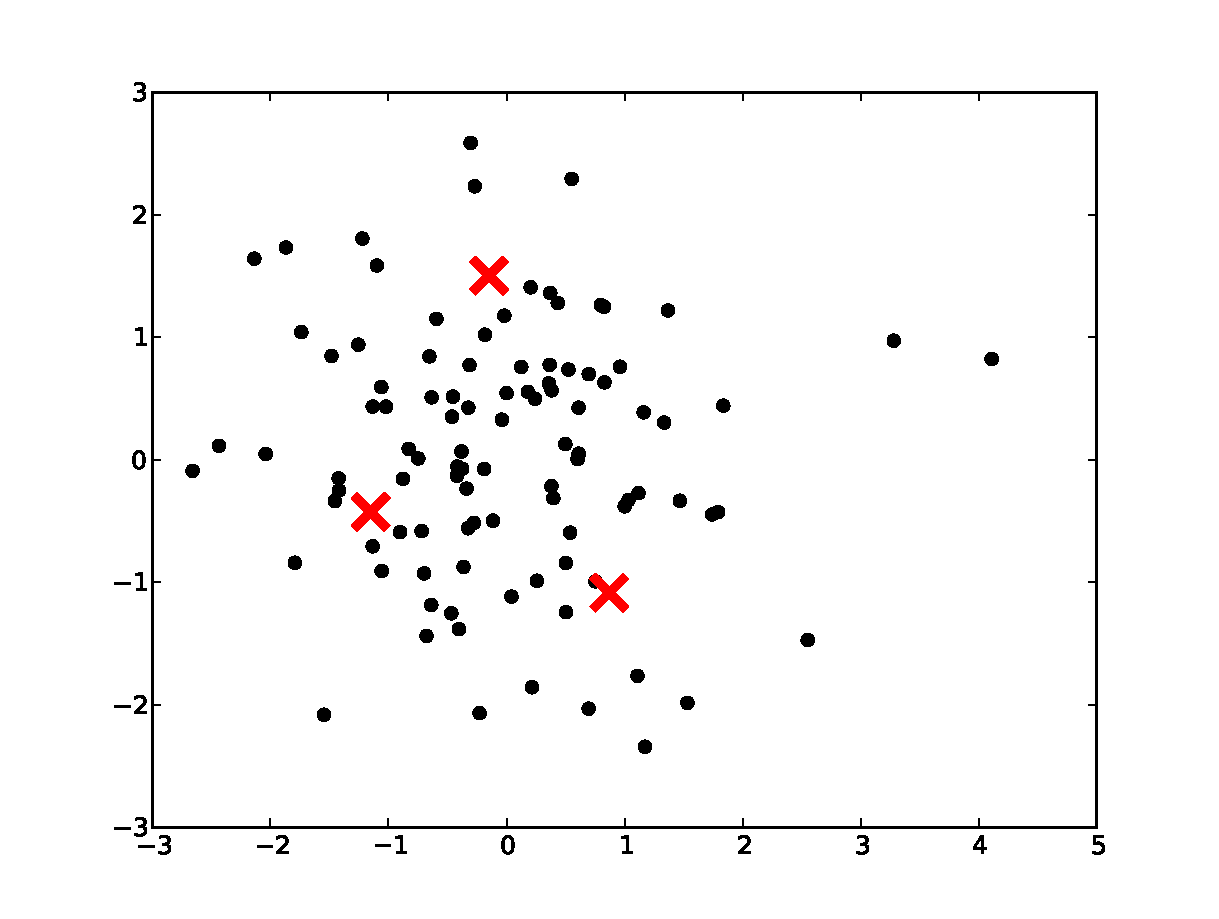
\includegraphics[width=5.5cm]{example_2d_original}
  \caption{A 2-dimensional example of $50$ points (black circles)
    drawn from $\mathcal{N}(\boldsymbol{0},I)$ and $3$
    prototypes (red stars) drawn from the same pdf.}
  \label{fig:toy_example_2d}
\end{figure}

\begin{figure}
  \centering
  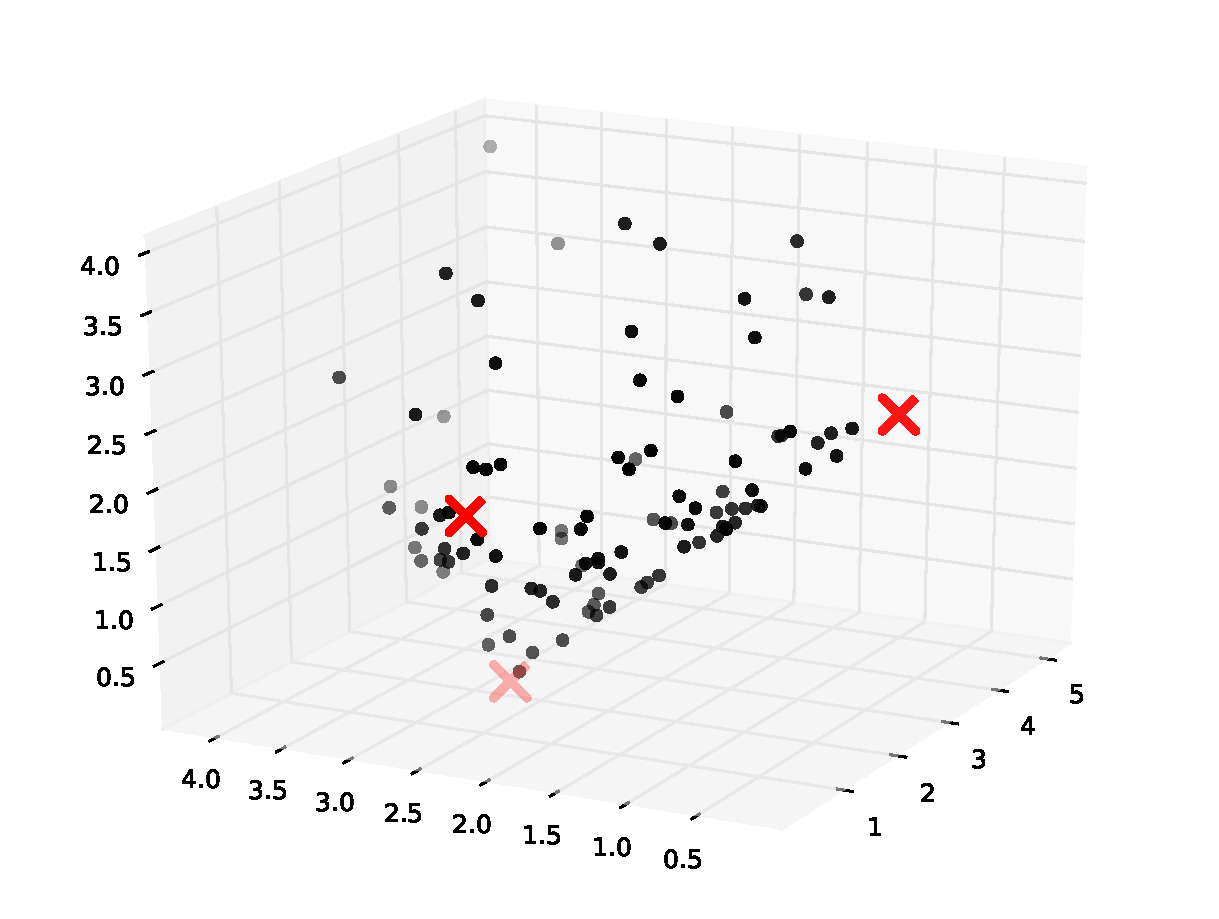
\includegraphics[width=5.5cm]{example_2d_dissimilarity}
  \caption{The dissimilarity projection of the dataset and prototypes
    of Figure~\ref{fig:toy_example_2d}.}
  \label{fig:toy_example_2d_projected}
\end{figure}

The selection of the prototypes according to different policies is
explained in Section~\ref{sec:policies}. For SFF we chose $c = 3$ in
order to have high probability ($>0.95$) of accurately representing $S$ through
the subset. Each dataset was projected in the dissimilarity space. The
correlation $\boldsymbol{\rho}$ between distances in the original
space and the corresponding distances in the projected space was
estimated by computing $50$ repetitions of the simulated dataset. The
average correlation and one standard deviation for each prototype
selection strategy are shown in Figure~\ref{fig:example_2d_policies}.

\begin{figure}
  \centering
  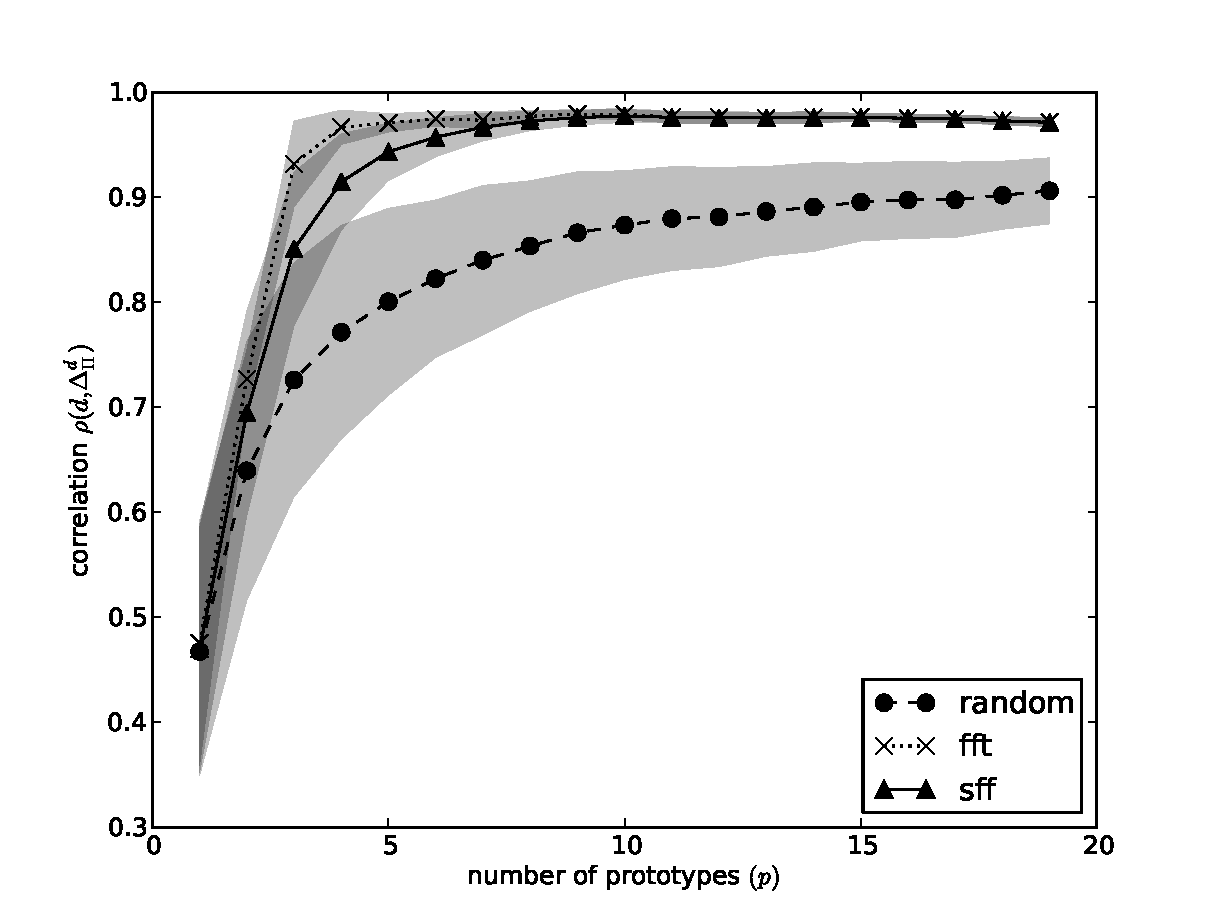
\includegraphics[width=7.5cm,height=5.0cm]{simulated_data_correlation_policies}
  \caption{Average correlation between $d$ and $\Delta_{\Pi}^d$ across
    different prototype selection policies and different numbers of
    prototypes.}
  \label{fig:example_2d_policies}
\end{figure}

In this simulated dataset both SFF and FFT performed significantly
better than the random selection, on average. FFT showed a small
advantage over SFF when $p<10$.


\subsection{Tractography data}
\label{sec:experiments_tractography_data}
We estimated the dissimilarity representation over tractography data
from dMRI recordings of the MRI facility at the MRC Cognition and
Brain Sciences Unit, Cambridge UK. The dataset consisted of $12$
healthy subjects; $101$ ($+1$, i.e. $b=0$) gradients; $b$-values from
0 to 4000; voxel size: $2.5 \times 2.5 \times 2.5 mm^3$. In order to
get the tractography we computed the single tensor reconstruction
(DTI) and created the streamlines using EuDX, a deterministic tracking
algorithm~\cite{garyfallidis2012towards} from the DiPy
library~\footnote{\url{http://www.dipy.org}}. We obtained two
tractographies using $10^4$ and $3 \times 10^6$ random seed
respectively. The first tractography consisted of approximately $10^3$
streamlines and the second one of $3 \times 10^5$ streamlines. An
example of a set of prototypes from the largest tractography is shown
in Figure~\ref{fig:streamlines}.

As the distance between streamlines we chose one of the most common,
i.e. the symmetric minimum average distance
from~\cite{zhang2008identifying} defined as $d(X_a,X_b) =
\frac{1}{2}(\delta(X_a,X_b) + \delta(X_b,X_a))$ where
\begin{equation}
  \label{eq:mam_distance}
  \delta(X_a,X_b) = \frac{1}{|X_a|} \sum_{\mathbf{x}_i \in X_a}
    \min_{\mathbf{y} \in X_b} ||\mathbf{x}_i - \mathbf{y}||_2.
\end{equation}

As it is shown in Figure~\ref{fig:correlation_1K} for the case of a
tractography of $10^3$ streamlines both FFT and SFF ($c = 3$) had
significantly higher correlation than the random sampling for all
numbers of prototypes considered. We confirmed that the SFF selection
policy is an accurate approximation of the FFT policy for
tractographies. Moreover we noted that after $15-20$ prototypes the
correlation reaches approximately $0.95$ on average ($50$ repetitions)
and then slightly decreases indicating that a little number of
prototypes is sufficient to reach a very accurate dissimilarity
representation.

Figure~\ref{fig:correlation_300K} shows the correlation for
SFF and the random policy when the tractography has $3 \times 10^5$
streamlines, i.e. the standard size of a tractography from current
dMRI recording techniques. In this case FFT is impractical to be computed
because it requires approximately $15$ minutes on a standard desktop computer
for a single repetition when $p=50$. The cost of computing SFF is
instead the same of the case of $10^3$ streamlines, as its
computational cost depends only on the number of prototypes. It took
$\approx 2$ seconds on standard desktop computer when $p=50$ to compute one
repetition. We observed that for $3 \times 10^5$ streamlines SFF
significantly outperformed the random policy and reached the highest
correlation of $0.96$ on average ($50$ repetitions) for $15-25$
prototypes.

Note that the figures presented in this section refers to data from
subject $1$ of the dMRI dataset. We conducted the same experiments on
other subjects obtaining equivalent results. The code to reproduce all
the experiments is available
at~\url{https://github.com/emanuele/prni2012_dissimilarity} under an open source
license.

\begin{figure}
  \centering
  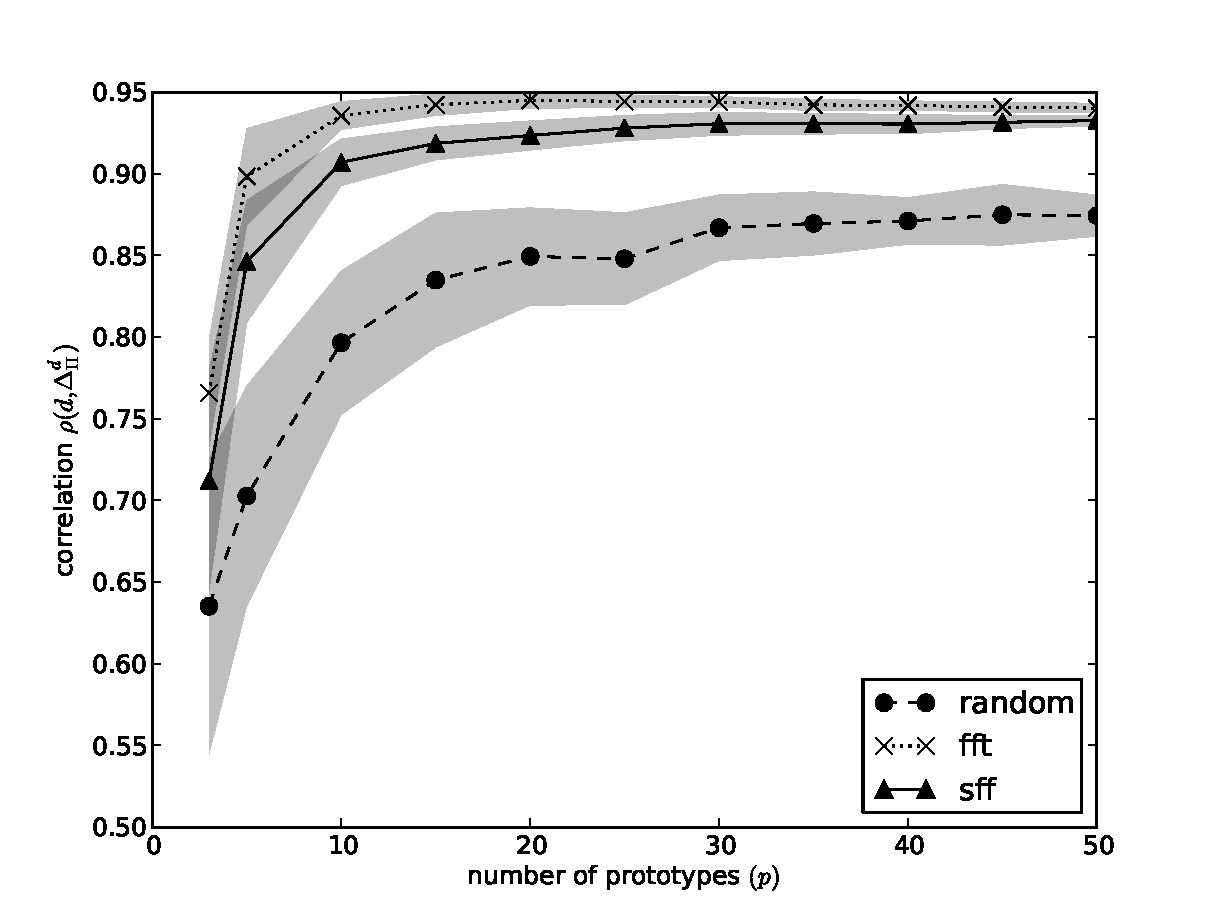
\includegraphics[width=8.5cm,height=5.5cm] {tracks_1K_correlation_policies}
  \caption{The correlation between of $d$ and $\Delta_{\Pi}^d$ over a
    $10^3$ streamlines tractography for different prototype selection
    policies.}
  \label{fig:correlation_1K}
\end{figure}


\begin{figure}
  \centering
  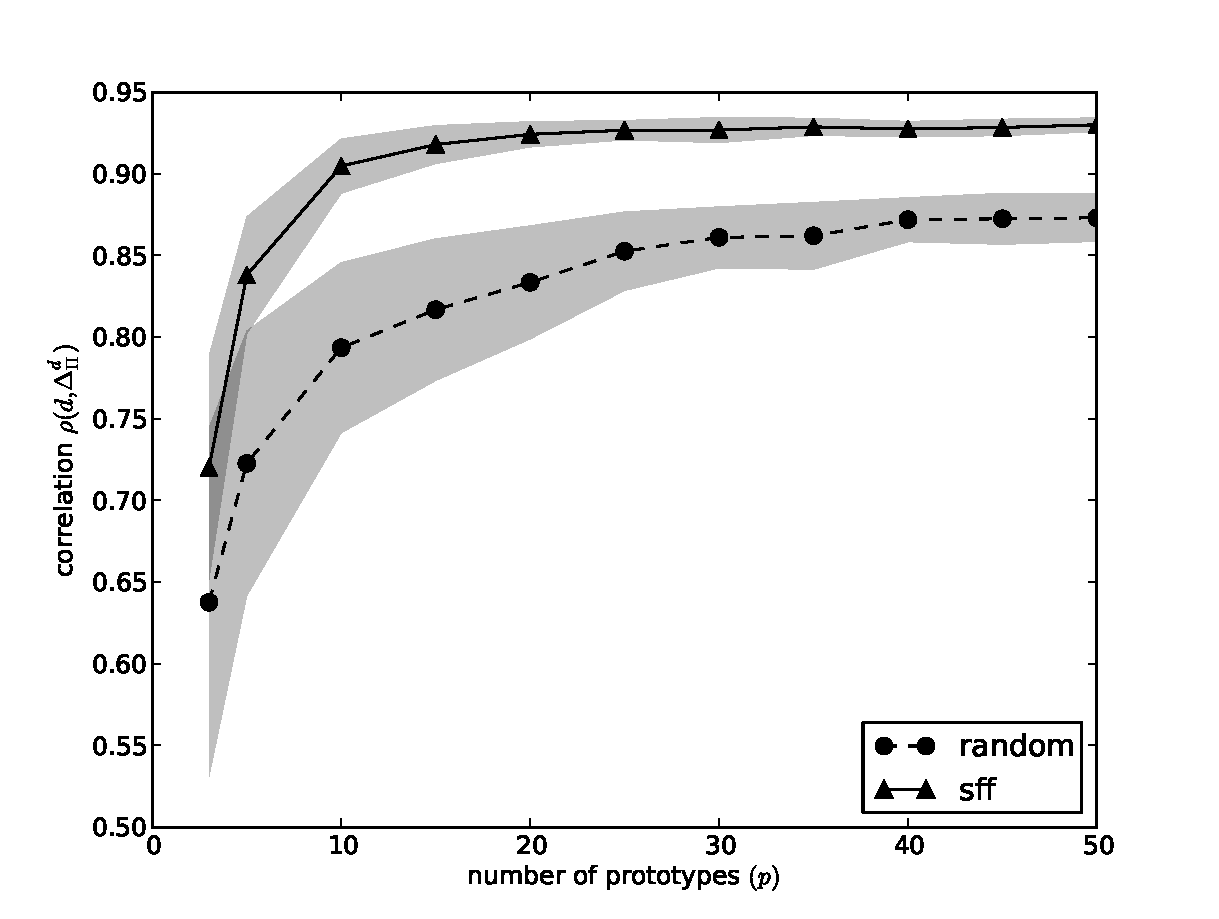
\includegraphics[width=8.5cm,height=5.5cm] {tracks_300K_correlation_policies}
  \caption{The correlation between of $d$ and $\Delta_{\Pi}^d$ for a
    full tractography of $3 \times 10^5$ streamlines for the random and SFF
    prototype selection policies.}
  \label{fig:correlation_300K}
\end{figure}


%%% Local Variables: 
%%% mode: latex
%%% TeX-master: "nguyen_dissimilarity"
%%% End: 
